\section{Trainings- und Testmenge}
\label{sec:synthetischeDaten}
\label{sec:testdaten}
Die Modelle werden auf Basis von aufgenommenen Daten trainiert und getestet. Die Aufnahmen beinhalten die 5 Handgestentypen, die mit unterschiedlichen Lichtverhältnissen aufgenommen wurden. Die Lichtverhältnisse
sind durch verschiedene Lichtquellen und Ausführungsdistanzen der Handgeste zur Kamera entstanden. Die Handgesten wurden mit der flachen Hand oder mit dem Finger in verschiedenen Geschwindigkeiten ausgeführt.
Die Datenmenge umfasst insgesamt 4792 Handgesten.
\newline
\newline
Listing \ref{lst:sampleGesture} zeigt ein Beispiel einer gespeicherten Handgeste von Links nach Rechts. Abbildung \ref{fig:sample_gesture} illustriert die Handgeste als Graustufenbild.
Jedes Bild wird durch einen Komma separierten Vektor von Zahlen dargestellt. Die letzte Zahl ist die Beschriftung der Handgeste.
\begin{lstlisting}[label=lst:sampleGesture,caption={Beispiel einer gespeicherten Handgeste von Links nach Rechts.}]
    ...
    665,683,669,690,627,670,672,611,557,1
    662,679,657,676,564,592,633,467,415,1
    645,653,583,627,549,483,598,474,230,1
    576,444,269,488,251,209,352,184,187,1
    361,254,123,343,130,82,304,83,36,1
    131,69,41,120,34,39,72,25,30,1
    49,71,174,61,45,206,40,45,110,1
    111,242,473,113,195,467,122,210,343,1
    272,559,637,304,518,639,401,553,562,1
    566,646,654,592,580,654,634,618,602,1
    ...
\end{lstlisting}
Um die Datenmenge zu vergrößern, können synthetische Daten erzeugt werden. Dabei werden aus einer aufgenommenen Handgeste Variationen durch Rotation und Rauschen generiert. Außerdem können Helligkeiten,
Kontraste und Gamma verändert werden \cite{venzkeArticle}.
\newline
\newline
Als Testmenge wird ein Teil der Datenmenge bezeichnet, der nicht zum Trainieren verwendet wird. Kubik hat Testdaten unter verschiedenen Lichtverhältnissen und Entfernungen zur Kamera aufgenommen. Klisch hat
daraus eine Testmenge erstellt, die von Klisch und Giese zur Verifikation verwendet wurden \cite{klischThesis, gieseThesis}. Klisch definiert die Klassifizierungsgenauigkeit gemäß \ref{klisch_metric}. Die
Klassifizierungsgenauigkeit ist das Verhältnis zwischen der Anzahl an korrekt klassifizierten Handgesten und der Anzahl der Einträge in der Testmenge.
\begin{align}
    accuracy = \frac{\#true\ positives}{\#total\ gestures}
    \label{klisch_metric}
\end{align}
\begin{figure}[h!]
    \centering
    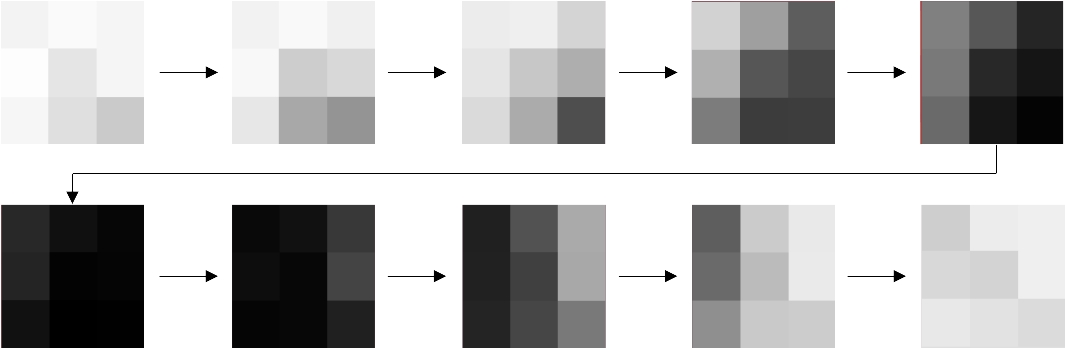
\includegraphics[width=\linewidth]{images/sample_gesture_total.jpg}
    \caption{Illustration der Handgeste von Links nach Rechts aus Listing \ref{lst:sampleGesture}.}
    \label{fig:sample_gesture}
\end{figure}